% THIS TEMPLATE IS A WORK IN PROGRESS

\documentclass[polish, a4paper]{article}
\usepackage[a4paper,left=3cm,right=3cm,top=3cm,bottom=1.5cm]{geometry}
\usepackage[T1]{fontenc}
\usepackage[polish]{babel}
\usepackage[utf8]{inputenc}
\usepackage{hyperref}
\usepackage{fancyhdr}
\usepackage{float}
\usepackage{graphicx}
\usepackage{titling}
\usepackage{wasysym}
\usepackage{caption}
\usepackage{pgfplots}
\usepackage{pgfplotstable}
\usepackage{filecontents}
\usepackage{csvsimple}
\usepackage{textcomp}
\usepackage{gensymb}
\usepackage{etoolbox}
%\usepackage{siunitx}
\graphicspath{ {./} }
\pagestyle{fancy}

\setlength{\droptitle}{-1in}

%\lhead{\includegraphics[width=0.2\textwidth]{nyush-logo.pdf}}

  \lhead{Maciej Kaszkowiak}
  \chead{Ćwiczenie 122}
  \rhead{Lab 4,
  151856}


%%%% PROJECT TITLE
\title{Wyznaczanie prędkości rozchodzenia się fal akustycznych w prętach \\
        \Large \emph{Ćwiczenie nr 122 z działu Mechanika}}

%%%% NAMES OF ALL THE STUDENTS INVOLVED (first-name last-name)
\author{Maciej Kaszkowiak, Lab 4, 151856}

\date{\vspace{-5ex}} %NO DATE


\begin{document}
\maketitle
%\thispagestyle{titlepage}

\section{Cel ćwiczenia}
Przeprowadzone ćwiczenie ma następujący cel:
\begin{enumerate}
\item{Wyznaczenie prędkości rozchodzenia się fal akustycznych w prętach wykonanych z różnych
materiałów oraz modułów Younga tych materiałów. }
\end{enumerate}
\section{Wstęp teoretyczny}

Fale akustyczne są rodzajem fal mechanicznych, które powstają w wyniku wychylenia elementu ośrodka sprężystego ze stanu równowagi. W konsekwencji tego, drgania te są przekazywane pomiędzy poszczególnymi cząsteczkami ośrodka, powodując przemieszczanie się zaburzenia, a tym samym, fali. Wyróżniamy dwa rodzaje fal akustycznych: podłużne i poprzeczne. Te pierwsze mogą rozchodzić się we wszystkich ośrodkach materialnych, zaś te drugie tylko w ciałach stałych lub bardzo lepkich cieczach. Prędkość rozchodzenia się fal akustycznych jest zależna od sprężystości i gęstości ośrodka. W przypadku, gdy średnica pręta jest porównywalna do długości fali akustycznej lub mniejsza, drgania nie mają charakteru czysto podłużnego. W niniejszym sprawozdaniu będziemy zajmować się wyznaczaniem prędkości rozchodzenia się fal akustycznych w prętach.

\begin{figure}[H]
\centering
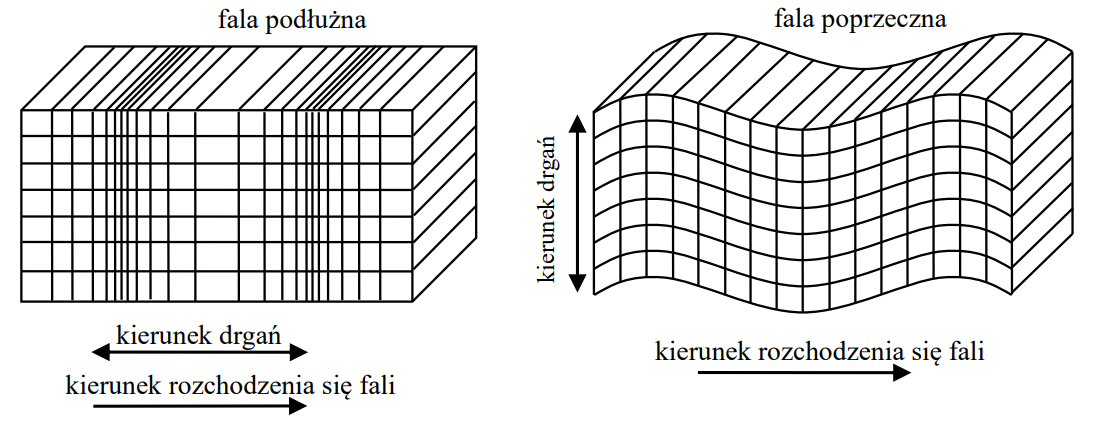
\includegraphics[width=0.8\textwidth]{fale.png}
\caption{Uproszczony obraz fal mechanicznych: podłużnej i poprzecznej}
\end{figure}

\section{Przebieg ćwiczenia}

Włączyliśmy urządzenia na stanowisku oraz komputer. Otworzyliśmy program Cassylab służący do przeprowadzania pomiarów.
Dla wszystkich czterech dostępnych prętów (z miedzi, stali, mosiądzu oraz aluminium):
\begin{enumerate}
\item{Umieściliśmy pręt w uchwycie oraz dosunęliśmy go do czujnika piezoelektrycznego.}
\item{Włączylismy program Cassylab w stan czuwania.}
\item{Za pomocą młoteczka delikatnie uderzyliśmy w środek powierzchni poprzecznej pręta.}
\item{Odczytaliśmy czas $t_1$ oraz $t_n$ dla ostatniego impulsu możliwego do zmierzenia.}
\end{enumerate}
Punkty 2-4 powtórzyliśmy do uzyskania czterech dokładnych pomiarów dla pręta.

Ponadto dla każdego pręta zmierzyliśmy długość oraz średnicę. 
Średnicę zmierzyliśmy w trzech różnych miejscach pręta w celu uzyskania uśrednionej wartości.

\begin{figure}[H]
\centering
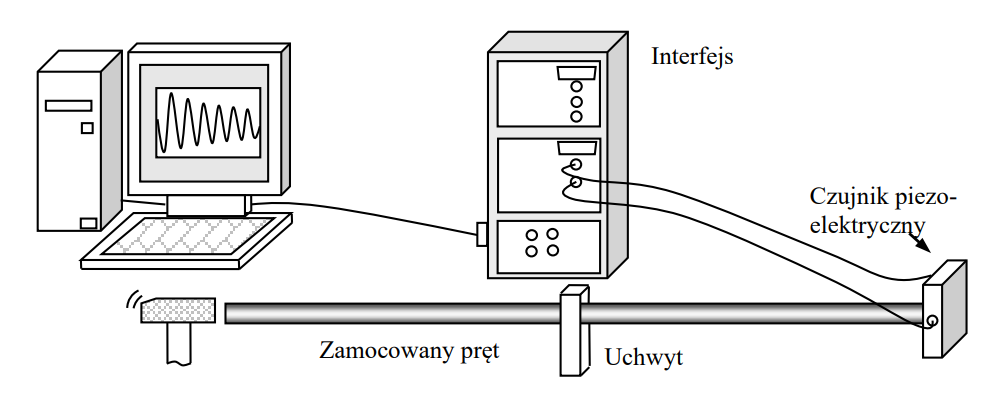
\includegraphics[width=0.8\textwidth]{stanowisko.png}
\caption{Schemat stanowiska pomiarowego.}
\end{figure}

\section{Wyniki pomiarów}


\begin{table}[H]
    \centering
        \csvreader[head to column names, 
        tabular=|l|l|l|l|,
        late after last line=\\\hline,
        late after line=\\\hline,
        table head=\hline Nr pomiaru & $t_1$ (ms) & $t_8$ (ms) & $\Delta t$ (ms) \\\hline]{mloteczek.csv}{}{\csuse{nr} & \csuse{Stal_t1} & \csuse{Stal_t8} & \csuse{Stal_ms}}
    \caption{Pomiary czasu rozchodzenia się fali w stalowym pręcie.}
\end{table}

\begin{table}[H]
    \centering
        \csvreader[head to column names, 
        tabular=|l|l|l|l|,
        late after last line=\\\hline,
        late after line=\\\hline,
        table head=\hline Nr pomiaru & $t_1$ (ms) & $t_9$ (ms) & $\Delta t$ (ms) \\\hline]{mloteczek.csv}{}{\csuse{nr} & \csuse{Aluminium_t1} & \csuse{Aluminium_t9} & \csuse{Aluminium_ms}}
    \caption{Pomiary czasu rozchodzenia się fali w aluminiowym pręcie.}
\end{table}

\begin{table}[H]
    \centering
        \csvreader[head to column names, 
        tabular=|l|l|l|l|,
        late after last line=\\\hline,
        late after line=\\\hline,
        table head=\hline Nr pomiaru & $t_1$ (ms) & $t_6$ (ms) & $\Delta t$ (ms) \\\hline]{mloteczek.csv}{}{\csuse{nr} & \csuse{Miedz_t1} & \csuse{Miedz_t6} & \csuse{Miedz-ms}}
    \caption{Pomiary czasu rozchodzenia się fali w miedzianym pręcie.}
\end{table}

\begin{table}[H]
    \centering
        \csvreader[head to column names, 
        tabular=|l|l|l|l|,
        late after last line=\\\hline,
        late after line=\\\hline,
        table head=\hline Nr pomiaru & $t_1$ (ms) & $t_6$ (ms) & $\Delta t$ (ms) \\\hline]{mloteczek.csv}{}{\csuse{nr} & \csuse{Mosiadz_t1} & \csuse{Mosiadz_t6} & \csuse{Mosiadz_ms}}
    \caption{Pomiary czasu rozchodzenia się fali w mosiężnym pręcie.}
\end{table}

\begin{table}[H]
    \centering
        \csvreader[head to column names, 
        tabular=|l|l|l|l|l|l|,
        late after last line=\\\hline,
        late after line=\\\hline,
        table head=\hline Materiał & $l$ (cm) & $\diameter_1$ (cm) & $\diameter_2$ (cm) & $\diameter_3$ (cm) & $\overline{\diameter}$ (cm) \\\hline]{dlugosci.csv}{}{\csuse{material} & \csuse{dlugosc_cm} & \csuse{pomiar_1} & \csuse{pomiar_2} & \csuse{pomiar_3} & \csuse{srednica_cm} }
    \caption{Pomiary długości $l$ oraz średnicy $\diameter$ dla poszczególnych prętów.}
\end{table}

Pomiar długości został wykonany z dokładnością do $1$ mm. Pomiary średnicy zostały wykonane z dokładnością $0.2$ mm. Ze względu na przeoczenie w trakcie wykonywania pomiarów, nie zmierzyliśmy masy poszczególnych prętów. W celu przeprowadzenia obliczeń posłużyliśmy się teoretyczną wartościami gęstości:

\begin{table}[H]
    \centering
        \csvreader[head to column names, 
        tabular=|l|l|l|,
        late after last line=\\\hline,
        late after line=\\\hline,
        table head=\hline Materiał & Gęstość $\rho$ ($\frac{kg}{m^3}$) & $\Delta \rho$ \\\hline]{gestosc.csv}{}{\csuse{material} & \csuse{gestosc_kg_m} & \csuse{niepewnosc} }
    \caption{Teoretyczne wartości gęstości dla poszczególnych materiałów.}
\end{table}

Pragniemy w tym miejscu zauważyć, że teoretyczne wartości odbiegają od rzeczywistych. Dla stopów stali oraz mosiądzu występują przedziały gęstości, spośród których musieliśmy wybrać jedną wartość. Dla mosiądzu wybraliśmy wartość środkową z dopuszczalnego przedziału gęstości. Dla stali wybraliśmy powszechnie przyjmowaną wartość z niepewnością odwzorowującą dopuszczalny przedział gęstości. Nie byliśmy w stanie pozyskać rzeczywistych pomiarów masy od innej grupy. W przypadku posiadania pomiarów masy, do wyznaczenia gęstości posłużylibyśmy się następującymi wzorami:

\begin{equation}
\rho = \frac{m}{V}
\end{equation}


\begin{equation}
V = \pi \cdot (\frac{d}{2})^2 \cdot L
\end{equation}

\begin{equation}
V = \frac{\pi}{4} d^2 L
\end{equation}

\begin{equation}
\rho = \frac{4m}{\pi d^2 L}
\end{equation}

Dla powyższego wzoru na gęstość niepewność wynosi $\Delta \rho$ z wykorzystaniem rachunku różniczkowego:

\begin{equation}
\Delta \rho = \rho \cdot ( \frac{\Delta m}{m} + \frac{\Delta L}{L} + \frac{2\Delta d}{d})
\end{equation}

\section{Opracowanie wyników}

Wykorzystując wzór na prędkość rozchodzenia się podłużnych fal sprężystych w pręcie:

\begin{equation}
v = \sqrt{\frac{E}{\rho}}
\end{equation}
Możemy wyprowadzić wzór na moduł Younga $E$:
\begin{equation}
E = v^2 \cdot \rho
\end{equation}
Gdzie prędkość rozchodzenia się podłużnych fal sprężystych w pręcie możemy obliczyć poprzez:
\begin{equation}
v = \frac{2l}{\Delta t}
\end{equation}
$l$ oznacza długość pręta, natomiast $\Delta t$ oznacza czas przebiegu zaburzenia w pręcie (tam i z powrotem).

\begin{table}[H]
    \centering
        \csvreader[head to column names, 
        tabular=|l|l|l|l|l|l|,
        late after last line=\\\hline,
        late after line=\\\hline,
        table head=\hline Materiał & Długość (cm) & $\Delta t$ (ms) & V ($\frac{m}{s}$) & $\rho$ ($\frac{kg}{m^2}$) & Moduł $E$ ($GPa$)  \\\hline]{obliczenia.csv}{}{\csuse{material} & \csuse{dlugosc_cm} & \csuse{delta_t_ms} &  \csuse{v_m_s} & \csuse{gestosc_kg_m2} & \csuse{young_GPa} }
    \caption{Obliczone wartości modułu Younga dla poszczególnych prętów.}
\end{table}


\begin{table}[H]
    \centering
        \csvreader[head to column names, 
        tabular=|l|l|l|l|l|,
        late after last line=\\\hline,
        late after line=\\\hline,
        table head=\hline Materiał & $V$ ($\frac{m}{s}$) & Teoretyczne $V$ & Moduł Younga $E$ ($GPa$) & Teoretyczne $E$  \\\hline]{obliczenia.csv}{}{\csuse{material} & \csuse{v_m_s} & \csuse{teor_v_20c} & \csuse{young_GPa} & \csuse{teor_young_GPa} }
    \caption{Zestawienie obliczonych wartości z wartościami teoretycznymi dla poszczególnych prętów. Wartości teoretyczne przyjęte dla temperatury 20 stopni Celsjusza.}
\end{table}

TODO: niepewność pomiarowa modułu Younga oraz prędkości V.

%% material,dlugosc_cm,delta_t_ms,v_m_s,teor_v_20c,teor_young_GPa,gestosc_kg_m2,young_GPa 
\section{Wnioski}

TODO: Pomiary złe. Prędkość fali zbliżona do teoretycznej. Miedź i aluminium zgadzają się z teorią. Mosiadz i stal lekki rozjazd (bo gęstość z neta). Gdyby nie gęstość to dobrze by wszystko legancko wyszło. Błąd paralaksy. XD 

\section{Bibliografia}

\begin{enumerate}
    \item {\emph{Wyznaczanie prędkości rozchodzenia się fal akustycznych w prętach } (Krzysztof Łapsa)}
\end{enumerate}


\end{document}
